\documentclass{article}

% if you need to pass options to natbib, use, e.g.:
\PassOptionsToPackage{numbers, compress}{natbib}
% before loading neurips_2026

% The authors should use one of these tracks.
% Before accepting by the NeurIPS conference, select one of the options below.
% 0. "default" for submission
\usepackage{neurips_2026}
% the "default" option is equal to the "main" option, which is used for the Main Track with double-blind reviewing.
% 1. "main" option is used for the Main Track
%  \usepackage[main]{neurips_2026}
% 2. "position" option is used for the Position Paper Track
%  \usepackage[position]{neurips_2026}
% 3. "eandd" option is used for the Evaluations & Datasets Track
 % \usepackage[eandd]{neurips_2026}
 % if you need to opt-in for a single-blind submission in the E&D track:
 %\usepackage[eandd, nonanonymous]{neurips_2026}
% 4. "creativeai" option is used for the Creative AI Track
%  \usepackage[creativeai]{neurips_2026}
% 5. "sglblindworkshop" option is used for the Workshop with single-blind reviewing
 % \usepackage[sglblindworkshop]{neurips_2026}
% 6. "dblblindworkshop" option is used for the Workshop with double-blind reviewing
%  \usepackage[dblblindworkshop]{neurips_2026}

% After being accepted, the authors should add "final" behind the track to compile a camera-ready version.
% 1. Main Track
%  \usepackage[main, final]{neurips_2026}
% 2. Position Paper Track
%  \usepackage[position, final]{neurips_2026}
% 3. Evaluations & Datasets Track
 % \usepackage[eandd, final]{neurips_2026}
% 4. Creative AI Track
%  \usepackage[creativeai, final]{neurips_2026}
% 5. Workshop with single-blind reviewing
%  \usepackage[sglblindworkshop, final]{neurips_2026}
% 6. Workshop with double-blind reviewing
%  \usepackage[dblblindworkshop, final]{neurips_2026}
% Note. For the workshop paper template, both \title{} and \workshoptitle{} are required, with the former indicating the paper title shown in the title and the latter indicating the workshop title displayed in the footnote.
% For workshops (5., 6.), the authors should add the name of the workshop, "\workshoptitle" command is used to set the workshop title.
% \workshoptitle{WORKSHOP TITLE}

% "preprint" option is used for arXiv or other preprint submissions
%  \usepackage[preprint]{neurips_2026}

% to avoid loading the natbib package, add option nonatbib:
%    \usepackage[nonatbib]{neurips_2026}

\usepackage[utf8]{inputenc} % allow utf-8 input
\usepackage[T1]{fontenc}    % use 8-bit T1 fonts
\usepackage{hyperref}       % hyperlinks
\usepackage{url}            % simple URL typesetting
\usepackage{booktabs}       % professional-quality tables
\usepackage{amsmath,amssymb,amsfonts}       % blackboard math symbols
\usepackage{nicefrac}       % compact symbols for 1/2, etc.
\usepackage{microtype}      % microtypography
\usepackage{xcolor}         % colors
\usepackage{graphicx} % Include figure files
\graphicspath{{figures/}} % Path to your figures
\usepackage{textcomp}
\usepackage{listings}
\usepackage{cleveref}
\usepackage{subcaption}
\usepackage[most]{tcolorbox}
\usepackage{tikz}
\usepackage{wrapfig}

\usepackage{amsthm}
\newtheorem{definition}{Definition}

% Inline project-board column label
\newcommand{\col}[1]{%
  \tikz[baseline=(X.base)]{%
    \node[draw=gray!80, fill=gray!10, rounded corners=2pt,
          inner sep=2pt,
          font=\scriptsize\sffamily] (X) {#1};%
  }%
}

% Note. For the workshop paper template, both \title{} and \workshoptitle{} are required, with the former indicating the paper title shown in the title and the latter indicating the workshop title displayed in the footnote. 
\title{Problem Reductions at Scale: Agentic Integration of Computationally Hard Problems}


% The \author macro works with any number of authors. There are two commands
% used to separate the names and addresses of multiple authors: \And and \AND.
%
% Using \And between authors leaves it to LaTeX to determine where to break the
% lines. Using \AND forces a line break at that point. So, if LaTeX puts 3 of 4
% authors names on sthe first line, and the last on the second line, try using
% \AND instead of \And before the third author name.


\author{%
  Xi-Wei Pan\thanks{Equal contribution.} \\
  Thrust of Advanced Materials \\
  The Hong Kong University of Science and Technology (Guangzhou) \\
  Guangdong, China \\
  \texttt{xiwei.pan@connect.hkust-gz.edu.cn}
  \And
  Shi-Wen An\footnotemark[1] \\
  Department of Information and Communication Engineering \\
  Institute of Science Tokyo, Tokyo, Japan \\
  Center for Advanced Intelligence Project (AIP), RIKEN \\
  \texttt{an.s.aa@m.titech.ac.jp} 
  \AND
  Jin-Guo Liu \\
  Thrust of Advanced Materials \\
  The Hong Kong University of Science and Technology (Guangzhou) \\
  Guangdong, China \\
  \texttt{jinguoliu@hkust-gz.edu.cn}
}


\begin{document}


\maketitle


\begin{abstract}
  Solving an NP-hard optimization problem often requires reformulating it for a specific solver---quantum hardware, a commercial optimizer, or a domain heuristic.
  A tool for polynomial-time reductions between hard problems would let practitioners route any supported problem to any supported solver through a single interface.
  Building such a library at scale, however, has remained out of reach.
  We show that \emph{harness engineering}, the practice of designing constraints, verification systems, and feedback loops that channel AI coding agents, can overcome this barrier.
  Our harness combines a no-code contribution route for domain experts, a multilayer verification stack ranging from type-level checks to agentic feature tests (AI agents role-playing as end users), and a fully automated implementation-review-integration pipeline.
  In about three months, we built a command-line tool backed by a library of 100+ problem types and 200+ reduction rules in over 170k lines of Rust.
  The result suggests that a well-engineered harness lets agents build well-tested software at a scale and pace beyond prior reduction-library efforts.
  Because the reduction graph composes transitively, a new solver registered for any single problem type instantly becomes available to every problem connected by a reduction path.
\end{abstract}



\section{Introduction}\label{sec:intro}

\subsection{Many Hard Problems, Few Solvers}

Combinatorial optimization problems arise throughout science and engineering~\cite{korte2008combinatorial,Schuetz2022PhysicsGNN}.
An airline needs to assign crews to flights~\cite{gopalakrishnan2005airline}.
A chip designer needs to allocate registers, commonly modeled as graph coloring in compilers~\cite{chaitin1981register}.
A logistics company needs to route delivery trucks~\cite{toth2014vehicle}.
Each of these is an instance of an NP-hard problem~\cite{karp1972,garey1979}, a class of problems for which no efficient general-purpose algorithm is known, but which can be solved in practice for moderate sizes by specialized solvers.

The difficulty is that each solver speaks its own narrow language.
SAT solvers~\cite{Een2003MiniSat, Biere2020Kissat} accept Boolean satisfiability instances.
Integer linear programming (ILP) engines like CPLEX~\cite{IBM2022CPLEX}, Gurobi~\cite{Gurobi2026}, and HiGHS~\cite{Huangfu2018HiGHS} require problems expressed as linear constraints over integer variables.
Semidefinite programming (SDP) relaxations tackle Max-Cut and graph bisection~\cite{GoemansWilliamson1995} but need a matrix formulation.
Beyond classical solvers, specialized hardware introduces additional formulations: D-Wave quantum annealers~\cite{glover2019} solve Quadratic Unconstrained Binary Optimization (QUBO), and Rydberg atom arrays~\cite{lucas2014, pichler2018, ebadi2022quantum} natively solve Maximum Independent Set on geometric graphs.
Physics-inspired methods scale further: graph neural networks solve QUBO at million-variable scale~\cite{Schuetz2022PhysicsGNN}, and hybrid quantum-GNN methods tackle the Traveling Salesman Problem~\cite{He2024QuantumTSP}.
These approaches still require a QUBO or Ising formulation as input.
A practitioner with a crew-scheduling problem cannot reach most of these solvers without first \emph{translating} the problem into a form the solver understands.

This translation is called a \emph{reduction}: an efficient algorithm that converts an instance of one problem into an instance of another and maps the
target's solution back to the source.
In other words, a reduction gives a uniform rule for solving any source instance via the corresponding target instance.
Each verified reduction is a bridge connecting a new problem to an existing solver.

\subsection{Bridging Problems to Solvers}

\begin{wrapfigure}{r}{0.4\textwidth}
  \vspace{-\baselineskip}
  \centering
  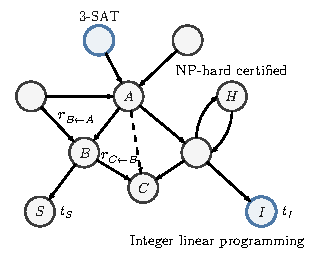
\includegraphics[width=0.4\textwidth]{figures/reduction-graph-concept.pdf}
  \caption{The reduction graph.  Two anchor problems are highlighted: \emph{3-SAT} at the top and \emph{Integer linear programming (ILP)} at the bottom right.  Edge labels are reduction overheads $r_{\cdot \leftarrow \cdot}$; node labels like $t_S$, $t_I$ denote the time complexity of the node's best known solver.}
  \label{fig:reduction-graph-concept}
  \vspace{-\baselineskip}
\end{wrapfigure}

A single reduction between two problems is a \emph{primitive reduction rule}.
Primitive rules collectively form a directed \emph{reduction graph} (\Cref{fig:reduction-graph-concept}): each node is a problem type, each directed edge is a primitive rule.
Every edge carries a \emph{reduction overhead}: a multivariate polynomial mapping the source's size measures to the target's; we write $r_{B \leftarrow A}$ for the overhead of the rule $A \to B$.

Reductions \emph{compose} along directed paths.
Chaining $A \to B$ and $B \to C$ along the central chain in \Cref{fig:reduction-graph-concept} yields a composite rule $A \to C$ with overhead $r_{C \leftarrow A} = r_{C \leftarrow B} \circ r_{B \leftarrow A}$.
Two kinds of paths play a special role, marked by the highlighted nodes in the figure.
3-SAT serves as the source of NP-hardness proofs: any path from 3-SAT to a problem~$H$ provides an NP-hardness argument for~$H$.
We say $H$ is \emph{NP-hard certified} by the reduction graph.
Integer linear programming (ILP) is backed by mature solvers: any path from a problem to ILP routes it to one of them, which is crucial for testing the correctness of reductions.
The target solver's time complexity, $t_I$ for ILP, thereby upper-bounds the end-to-end solving cost of any problem routed to it, up to reduction overhead.


\subsection{The Challenge}
\begin{wrapfigure}{r}{0.4\textwidth}
  \vspace{-\baselineskip}
  \centering
  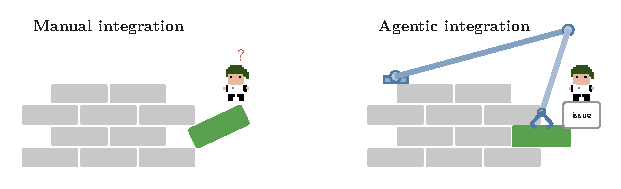
\includegraphics[width=0.3\textwidth]{figures/comic-integration.pdf}
  \caption{The integration problem.
    (a) A new reduction does not fit the library's conventions and cannot be integrated without learning the codebase.
    (b) The contributor files a structured issue; an agent handles implementation, review, and documentation.}
  \label{fig:comic}
  \vspace{-\baselineskip}
\end{wrapfigure}

Scaling an \emph{executable} reduction graph is an engineering problem.
The literature is far ahead of any implementation: Garey and Johnson~\cite{garey1979} catalogue over 300~NP-hard problems with reduction sketches, yet the largest software library (Appendix~\ref{sec:related}) covers fewer than 20.
Implementation and maintenance are the bottleneck, and two barriers in particular emerge.

\textbf{Convention drift.}
Every reduction rule must conform to the same interface, the same file layout, and the same test pattern.
Maintaining this uniformity across many contributions is precisely what human teams cannot do at scale: as contributors accumulate their own patterns, the codebase fractures.
A mathematician who understands a new reduction has no way to contribute it without first learning the implementation language and the project's conventions (\Cref{fig:comic}).

\textbf{Effort exhaustion.}
Every new entry demands the same lengthy checklist.
Adding a problem type requires resolving whether the problem is genuinely new or a known problem under a different name, writing a formal definition, and identifying the best known algorithm and its complexity.
Adding a reduction rule requires confirming that both endpoint problems exist, verifying the rule is novel and actually improves on existing routes, analyzing the reduction overhead, providing a correctness argument, implementing the forward and inverse maps, designing correctness tests, and documenting the reduction with a worked example.
Repeating this cycle for every entry exhausts even dedicated maintainers.

AI coding agents offer a way forward, but only when paired with a \emph{harness}---the engineered constraints, feedback loops, and automatic checks that channel agents toward reliable output~\cite{OpenAI2026HarnessEngineering}.
The engineer's job is no longer to write the code, but to design the harness that makes the agent's code trustworthy.
We build a domain-specific harness that addresses both \emph{convention drift} and \emph{effort exhaustion}; \Cref{sec:method} details its components.

\subsection{Contributions}

\begin{figure}
  \centering
  \includegraphics[width=\columnwidth]{figures/main.pdf}
  \caption{Overview.
    (a) Many solvers exist, and a problem can usually reach several of them through different reductions, but this knowledge is scattered across the literature without a unified executable framework.
    (b) A harness-engineered agentic workflow turns a structured GitHub issue into validated code through implementation and review agents under a four-layer verification stack.
    (c) Three months of this pipeline produced a reduction graph with 190 problem types and 265 rules; the inset shows growth over time.}
  \label{fig:overview}
\end{figure}

We make three contributions, each addressing one actor in the workflow:

\textbf{For domain experts.}
A no-code contribution route that turns a structured GitHub issue into validated implementation, with no familiarity with the implementation language needed.

\textbf{For maintainers.}
Our harness uses skills to guide agents through the full pipeline, from coding to the final review, under a layered correctness gate.
Maintainers are freed from routine work to focus on the intellectual work.

\textbf{For end users.}
The first comprehensive and executable library of computationally hard problem reductions: 200+ reductions among 100+ problem types and 170k lines of code, an inventory that would have taken years by hand but landed in three months with a small team and AI agents.

\begin{figure}[t]
  \centering
  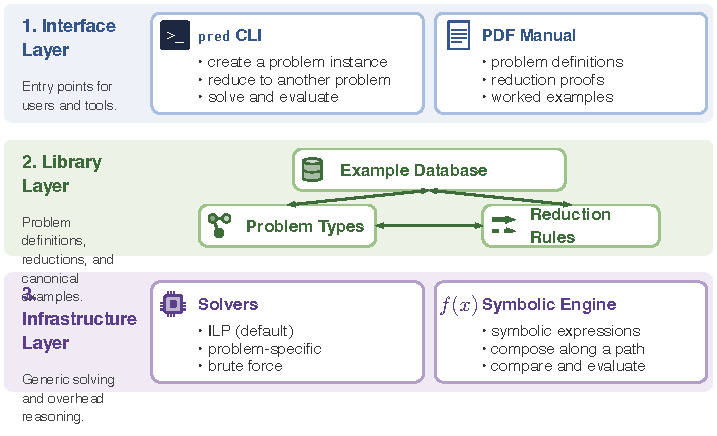
\includegraphics[width=0.85\columnwidth]{figures/library-architecture.pdf}
  \caption{System architecture.
    Three layers separate concerns: the interface layer (top) is what users and agents touch, the library layer (middle) holds the reduction graph itself, and the infrastructure layer (bottom) provides the computational backends---solvers for instances and a symbolic engine for overhead and complexity.}
  \label{fig:library-architecture}
\end{figure}

\section{System Architecture}\label{sec:architecture}

We implements the reduction graph as a Rust crate, organized in three layers (\Cref{fig:library-architecture}).

\subsection{Interfaces}\label{sec:user-interfaces}

The library exposes two interfaces, both designed for humans and AI agents: the \texttt{pred} command-line interface (CLI) and a PDF manual.

Through the CLI, \texttt{create} emits a problem instance as JSON, \texttt{reduce} transforms it along any reduction path, and the resulting JSON pipes into external solvers or downstream tools.
\texttt{solve} closes the loop for quick checks.
See Appendix~\ref{app:cli} for a worked session.

Compiled from Typst, the manual collects the library's formal mathematics: each problem and reduction has a definition, a worked example, a diagram, and a proof sketch.
Domain experts review it for correctness, and agents register a new entry whenever they add a model or rule, keeping code and mathematics in lockstep.

\subsection{Library Layer}\label{sec:graph-structure}

The library layer is a collection of problem types and the reduction rules between them.

\textbf{Problem types.}
Every problem type implements a uniform interface for problems, such as input domain, solution type and \emph{size measures}.
Each type defines its own size measures and \emph{best-known algorithm complexity}, for example, Maximum Independent Set (MIS) is parameterized by $|V|$ and $|E|$, with a known $O(1.1996^{|V|})$ algorithm~\cite{Xiao2017MIS}.
A problem type may have \emph{variants}: restricting the input domain to a narrower class preserves the combinatorial objective but can change the complexity.
Each variant occupies a distinct node in the reduction graph.
For instance, general MIS requires $O(1.1996^{|V|})$ time, whereas MIS on unit disk graphs admits a $2^{O(\sqrt{|V|})}$ algorithm, which is subexponential, unlike the general case~\cite{deBerg2020ETHTight}.

\textbf{Reduction rules.}
Each rule requires two mappings, a forward map and an inverse map. The forward map converts a source problem instance to a target problem instance.
After solving the target problem, the inverse map extracts source solutions from target solutions.
Each rule also carries a \emph{reduction overhead}: a set of multivariate polynomials mapping the source's size measures to the target's.
For example, the 3-SAT $\to$ MIS reduction creates one vertex per literal occurrence in the formula, yielding $O(L)$ vertices and $O(L^2)$ edges where $L$ is the total number of literal occurrences.

\textbf{Example database.}
Each problem type defines a canonical instance, such as the Petersen graph for Maximum Independent Set.
The same instance drives the test suite and serves as the worked example in the PDF manual.

\subsection{Infrastructure Layer}\label{sec:infrastructure}

The infrastructure layer provides the computational backends that the library layer builds on: backend solvers for exact verification, and a symbolic engine for analyzing computational complexity.

\textbf{Solvers.}
Every problem type needs a minimal but reasonably efficient solver, because testing requires solving each problem exactly.
Most types (e.g., Maximum Independent Set, Traveling Salesman, flow-shop scheduling) have a reduction path to ILP.
The default validation strategy reduces the problem to ILP and solves it with HiGHS~\cite{Huangfu2018HiGHS}, an open-source solver.
For problems without an ILP path, the library provides customized exact solvers that exploit problem structure---for example, functional-dependency closure for Minimum Cardinality Key~\cite{Lucchesi1978CandidateKeys}, and cycle enumeration with branch-and-bound for Partial Feedback Edge Set~\cite{Baharev2021FeedbackArcSet}.
The remaining problems fall back to brute-force enumeration on small instances.

\textbf{Symbolic engine.}
Both reduction overheads and algorithm complexities are represented as symbolic expressions.
The symbolic engine supports three operations: \emph{composition} substitutes one edge's output polynomial into the next edge's input, often used to determine the composite overhead of a multi-step reduction path; \emph{comparison} determines whether a symbolic expression has lower asymptotic growth than another, used for finding the cheapest reduction path; and \emph{evaluation} evaluates a symbolic expression.

Appendix~\ref{app:architecture} presents the engineering details of the Rust crate.

\subsection{Why Rust?}\label{sec:why-rust}

None of the maintainers had written Rust before this project.
The language was chosen in large part for properties that benefit agents.

\textbf{Strict compiler, actionable errors.}
Rust rejects many invalid programs before execution, and reports precise type, ownership, and lifetime errors.
These diagnostics give agents a concrete repair target.

\textbf{Fast feedback.}
Cargo provides a standard loop for building, testing, and formatting.
Incremental compilation and unit tests make that loop fast enough for agent iteration.


%======================================================================
%  SECTION 4: SKILLS AND AUTOMATION
%======================================================================
\section{Harness Design}\label{sec:method}

\subsection{Anatomy of the Harness}\label{sec:skills}

\begin{definition}[Harness System]
A \emph{harness system} constrains agent behavior through five components: a project specification auto-loaded into every agent session, a set of tools the agent may invoke, a progressively-disclosed knowledge base, a set of automation skills (executable checklists that compose the previous three into multi-step pipelines), and a set of advisor skills for human contributors onboarding.
\end{definition}

The five components address successive needs in an agent session: what conventions to follow, what actions to take, what domain knowledge to consult, and how to orchestrate these into workflows.

\textbf{Project specification} files at the repository root (\texttt{CLAUDE.md}, \texttt{AGENTS.md}) encode how to find the remaining four components and what conventions to follow.
Every agent session loads these files automatically on startup, ensuring that a new agent inherits the same conventions as every prior session, without human briefing.

\textbf{Tools} include command-line interfaces (CLI), model context providers (MCP), and external search services.
The CLI and the language's built-in test harness are the agent's hands.
In this project, the \texttt{pred} CLI lets agents create problem instances, run reductions, invoke solvers, and inspect topological connectivity in the reduction graph.
ArXiv MCP and web search retrieve references, and Typst compiles the PDF manual and its documentation artifacts.

\textbf{Knowledge base.}
Domain knowledge includes Garey and Johnson's catalogue~\cite{garey1979}, reference papers converted to Markdown for agent consumption, and reference implementations already in the codebase.
This body of material is too large to fit in a single agent context window.
The harness organizes this knowledge for \emph{progressive disclosure}~\cite{Nielsen2006ProgressiveDisclosure}: agents discover relevant files through search and read full content (formal definitions, proof sketches, worked examples) only when a specific task demands it.

\begin{figure}[t]
  \centering
  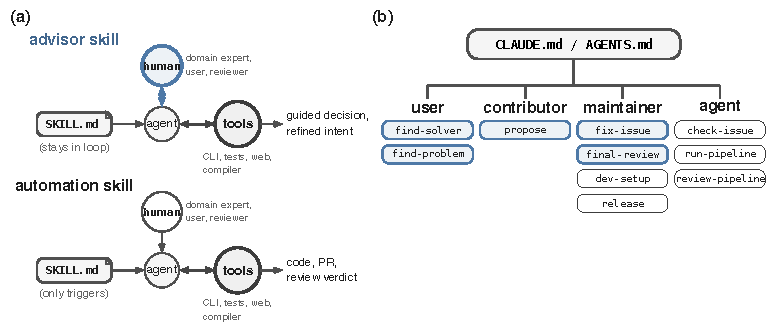
\includegraphics[width=\columnwidth]{figures/skill-map.pdf}
  \caption{Skills architecture.
    (a) The two skill kinds: \emph{advisor} skills keep humans in the loop with the agent throughout, while \emph{automation} skills run end-to-end once invoked. Other interactions with agents are omitted for clarity.
    (b) The skill catalogue, grouped by invoker (user, contributor, maintainer, or agent). Blue boxes are advisor skills; white boxes are automation skills.}
  \label{fig:skill-architecture}
  \end{figure}

Skills are plain-Markdown documents that orchestrate specification, tools, and knowledge into multi-step, repeatable workflows.
We divide skills into two kinds (\Cref{fig:skill-architecture}): \emph{automation skills} that agents execute end-to-end, and \emph{advisor skills} that bring humans into the loop at decision points.

\textbf{Automation skills} can include \emph{abstract} steps that traditional automation (Makefiles, shell scripts) cannot express: like ``implement the reduction algorithm''(\texttt{run-pipeline} skill in~\Cref{fig:skill-architecture}(b)), ``review the pull request for correctness''(\texttt{review-pipeline} skill) and ``make a new release''(\texttt{release} skill).
These steps require judgment and are interpreted by the agent using its own capabilities.
Unlike bare prompts, skills break a complex task into concrete, ordered steps small enough for an agent to execute faithfully, preventing the drift and omissions that occur when agents plan from scratch.

\textbf{Advisor skills} involve humans for two purposes: \emph{training} humans to use the library or contribute to it, and \emph{utilizing} humans for tasks agents cannot reliably perform, such as critical decisions, hard mathematical reasoning, and creative work like designing canonical examples.
\emph{Training} skills flatten the learning curve:
end users invoke \texttt{find-solver} skill (\Cref{fig:skill-architecture}(b)) to go from a real-world problem to a concrete solving strategy by exploring the reduction graph, or \texttt{find-problem} to discover what problems a given solver covers; contributors invoke \texttt{propose} skill to brainstorm a new problem or reduction in mathematical language and file a well-formed GitHub issue, with no programming required.
\emph{Utilizing} skills retain humans for critical correctness work: maintainers invoke \texttt{fix-issue} to identify and address quality issues such as unsound proofs or low-quality examples interactively, and \texttt{final-review} to catch dangerous commits or correctness gaps before merge.
These skills lower the usage barrier from ``knows the library'' to ``knows the problem,'' and the contribution barrier from ``knows the programming language'' to ``knows the mathematics.''

Appendix~\ref{app:skills} excerpts one skill of each kind: \texttt{propose} (advisor) and \texttt{add-rule} (automation).

\begin{wrapfigure}{r}{0.45\textwidth}
  \vspace{-\intextsep}
  \centering
  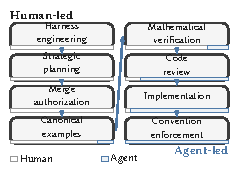
\includegraphics[width=\linewidth]{figures/delegation-spectrum.pdf}
  \caption{Delegation spectrum. Tasks sorted from fully human (top) to fully automated (bottom); bars show the human--agent split.}
  \label{fig:delegation-spectrum}
\end{wrapfigure}

\subsection{What Cannot Be Delegated}\label{sec:human-responsibilities}

Four responsibilities must remain with humans: \emph{selecting} which reduction to pursue, \emph{verifying} the algorithm's correctness, \emph{constructing} canonical examples, and \emph{authorizing} merges.
Selecting which rules to pursue requires understanding the needs of the community; the human is the information source.
Verifying the algorithm's correctness requires deep reasoning.
Reasoning ability of large language models degrades sharply with problem complexity~\cite{Mirzadeh2025GSMSymbolic,Shojaee2025IllusionOfThinking,Dziri2023FaithFate}. Research-level mathematics remains largely unsolved~\cite{Glazer2024FrontierMath,Paster2026HLE,Merrill2024ExpressivePower}.
Constructing canonical examples requires creative work; the human is the end user and the best judge.
Authorizing merges is security critical; a human with long-term memory must be responsible.

\Cref{fig:delegation-spectrum} summarizes the division of labor, sorted by how replaceable each task is by agents.

\subsection{Automation Pipeline}\label{sec:pipeline-overview}

\begin{figure*}[htbp]
  \centering
  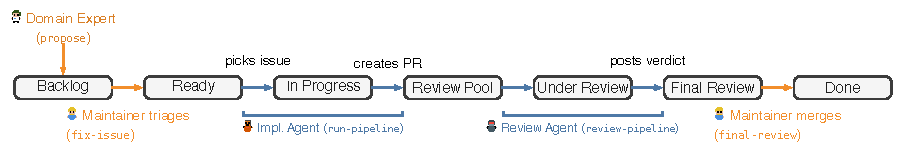
\includegraphics[width=\textwidth]{figures/pipeline.pdf}
  \caption{Contribution pipeline as a state machine on the GitHub project board.
    Each box is a board column (state); arrows show the single allowed transition direction.
    Four roles drive the flow: a \emph{domain expert} files issues (brown), a \emph{maintainer} triages and merges (orange), an \emph{implementation agent} picks issues and creates PRs (blue), and a \emph{review agent} runs parallel reviews and posts verdicts (teal).
    If any stage fails, the item moves to On~Hold (not shown) for human triage.}
  \label{fig:pipeline}
\end{figure*}

Adding a reduction to the graph involves six stages, mirrored as columns on a GitHub project board (\Cref{fig:pipeline}).
Each column is a state; progress flows left to right.
If any stage fails, the item moves to \col{OnHold} for human triage.
Four roles drive the flow: a domain expert files issues, a maintainer triages and merges, and two agents---one for implementation, one for review---handle the routine work in between.


\textbf{Stage~1: Propose} ( $\to$ \col{Backlog}).
A domain expert clones the repository and invokes the \texttt{propose} skill (\Cref{fig:skill-propose}) in Claude Code or a similar agentic coding tool.
The skill conducts a structured brainstorming session---one question at a time---to elicit the core content of the contribution: which problem or reduction rule to add, its formal definition, etc. The expert answers in mathematical language; no programming is required.
The agent runs a topology analysis to avoid duplicates and to identify high-value gaps in the reduction graph, then pre-validates the draft against Stage~2's quality checks.
The output is a structured GitHub issue filed into \col{Backlog}.

\textbf{Stage~2: Validate} (\col{Backlog} $\to$ \col{Ready}).
A maintainer invokes the \texttt{fix-issue} skill to triage each issue in \col{Backlog}.
The agent first evaluates the proposal along four dimensions: \emph{usefulness} (does a cheaper path already exist?), \emph{effort} (what is the effort to implement this rule?), \emph{correctness} (do cited references support the claims?), and \emph{writing quality} (are all symbols defined, all examples fully worked?).
It then auto-corrects mechanical failures (undefined symbols, missing metrics) and brainstorms substantive fixes with the maintainer interactively.
Only issues passing all four checks move to \col{Ready}.

\textbf{Stage~3: Implement} (\col{Ready} $\to$ \col{Review Pool}).
An implementation agent reads the \texttt{run-pipeline} skill, picks an issue automatically from \col{Ready} column, implements it\footnote{The engineering workflow builds on Superpowers~\cite{Obra2025Superpowers}}, submits a pull request (PR) and moves the issue to \col{Review Pool}---all in headless mode, no human in the loop.

\textbf{Stage~4: Review} (\col{Review Pool} $\to$ \col{Final Review}).
Similarly, a review agent reads the \texttt{review-pipeline} skill, claims an issue from \col{Review Pool}, moves it to \col{Under Review}, dispatches three read-only sub-agents: structural completeness, code quality, and agentic feature testing (AI agents role-playing as end users; \Cref{sec:verification}), and posts a review report on the PR and moves the issue to \col{Final Review}---all in headless mode.

\textbf{Stage~5: Merge} (\col{Final Review} $\to$ \col{Done}).
A maintainer invokes the \texttt{final-review} skill to review the PR.
Agent claims a PR from \col{Final Review}, checks the review report, performs mechanical fixes, walks the maintainer through the agentic verdict, and lets the maintainer make the final decision.
The maintainer either merges the PR to main branch (issue moved to \col{Done}) or holds the PR with a reason (issue moved to \col{OnHold}).

\textbf{Stage~6: Verify.}
The maintainer invites the domain expert who filed the original issue to a community call, and
walks through the PDF manual and CLI.
This closing-the-loop step catches errors invisible to automated tests: subtle misinterpretations of the problem statement or proof arguments.

Stages~3--4 (implement and review) run in \emph{headless mode} via OpenAI Codex~\cite{OpenAI2026Codex} (\texttt{gpt-5.4}, xhigh reasoning effort).
The remaining stages use Claude Code~\cite{Anthropic2025ClaudeCode} (\texttt{opus-4.6}) for interactive sessions with the maintainer and domain expert.
Anecdotally, we found \texttt{gpt-5.4} more reliable for code implementation and \texttt{opus-4.6} stronger in interactive dialogue, though we did not evaluate this systematically.

\subsection{Correctness Assurance}\label{sec:verification}

Correctness is enforced by six layers: issue review (Stage~2), compile-time type checks, unit tests, round-trip tests, \emph{agentic feature tests} (Stage~4) and manual verification (Stage 5 and 6). The first three are standard; we describe the two novel mechanisms below.

\textbf{Unit tests and round-trip tests.}
Unit tests cover individual problems, solvers, and helper functions.
Round-trip tests cover each reduction rule end-to-end: from a small canonical source instance, reduce, solve the target, lift the solution back, and compare against a direct solve of the source---an oracle the rule never invokes.

\textbf{Agentic feature tests.}
Libraries normally stabilize through community use, but a niche library cannot wait for that community to form.
Agentic feature tests approximate user feedback by simulating realistic use scenarios before real users arrive.
The mechanism has three phases.
First, the main agent launches a sub-agent in a \emph{fresh context window}---one that has never seen the implementation---and injects a \emph{user profile}: a structured persona with domain expertise and a concrete use case (Appendix~\ref{app:agent-profile}).
The fresh context is essential; an agent that has just written the code cannot objectively test it.
Second, the sub-agent role-plays the persona end-to-end: it reads only the project's documentation, picks a problem it recognizes from its domain, builds an instance with realistic data, discovers a reduction path through the CLI, solves, and verifies the result against its own expectation.
Third, the sub-agent steps out of character.
The main agent interviews it---what worked, what was confusing, where did the output diverge from expectation---and writes a structured report.
This report surfaces usability gaps, documentation omissions, and semantic errors that unit tests cannot reach.

In our practice, agentic feature tests caught most CLI command bugs, and some user-experience issues, e.g.\ the mismatch between the help text and the actual command output, which are never caught by the existing unit tests.

%======================================================================
%  SECTION 5: EVIDENCE
%======================================================================
\section{Evaluation}\label{sec:evidence}

We evaluate two questions. First, did our harness pipeline produce a substantive library? Second, is the resulting library useful to end users?

\subsection{Library Status}

\Cref{fig:overview}(c) summarizes the library at v0.5.0: 190~problem types (220 variants), 265~reduction rules, 129~types (68\%) with a reduction path to ILP, and 78 reachable from 3-SAT.
Each ILP path grants automatic solver access via the \texttt{pred} CLI; each 3-SAT path provides a tested NP-hardness argument backed by executable code rather than pen-and-paper proofs.
Growth is concentrated in the final phase: once the full skill-based pipeline came online at week~8.5, problem types went from 23 to 187 and reduction rules from 52 to 239 in under five weeks.
The phase-by-phase narrative is detailed in \Cref{app:phases}.

\subsection{End-User Utility}\label{sec:end-user-utility}

The library is itself an agent-callable tool via the \texttt{pred} CLI.
We measure whether catalog access improves how agents solve a problem stated in everyday language.
The instance: a manager splits a 150-person organization into two product teams; every pair of employees has a positive or negative compatibility score, and the goal is to maximize the sum of cross-team scores.
The agent's task is to pick the best algorithm for the problem and write the code that solves each instance.

To isolate the catalog's contribution, we compare four configurations that toggle \texttt{pred} access and web search independently (the four rows of \Cref{tab:end-user-eval}).
Each configuration is run on ten random instances (40 runs total), with solver wall-time capped at 90~s.
For each run we record three quantities: AI tokens spent on modelling, solver wall-time, and the objective value graded against the per-instance best (full setup in Appendix~\ref{app:end-user}).

\Cref{tab:end-user-eval} summarizes the outcomes.
The full \texttt{pred}+web configuration is the only one to match the per-instance best on every instance.
Bare AI matches it on 7 of 10; its worst run drops to $11{,}673$, a 9.8\% gap.
The intermediate configurations each suffer one or two large misses, all traceable to the same failure mode: the agent commits to a textbook integer-programming formulation, and its linear relaxation is too loose to close within 90~s.
\texttt{pred} access also speeds the solver up by a factor of $3$--$8$ at the cost of roughly $2{\times}$ more AI tokens.
The extra tokens go to reading the catalog; the speedup comes from the catalog's recommended endpoint---simulated annealing on the Ising form---which terminates in a single short call rather than a long branch-and-bound run.

\textbf{Solver-choice analysis.}
\Cref{tab:end-user-solver-table} reports the model and solver each agent settled on.
Without the catalog, agents scatter across HiGHS, Gurobi, OR-tools CP-SAT, dwave-neal / dwave-samplers SA, dwave-tabu, and ad-hoc local-search heuristics.
The catastrophic misses all come from integer- or mixed-integer routes whose linear relaxations are weak on dense signed-weight cut instances.
With the catalog, every run reformulates the instance as a signed-weight cut on a dense graph, follows the path through the spin-glass / QUBO family, and runs simulated annealing on the Ising form.
The catalog narrows the modelling choice to a single reformulation that the available solvers can handle within the time budget.

This experiment closes a loop in the paper: agents built the library, and the library now augments agents tackling new instances.

\begin{table}[h]
\caption{Outcomes on the team-split instance class (10~instances per configuration; 90~s solver-wall cap; 40~runs total). Agent: Claude Opus~4.7.
Higher objective is better; the per-instance best is the maximum across the four configurations on the same instance.}
\label{tab:end-user-eval}
\centering
\small
\begin{tabular}{@{}lccccc@{}}
\toprule
Configuration & Mean obj. & Min obj. & Best-match & Mean AI tokens & Mean solver s \\
\midrule
Bare AI                              & 12{,}431 & 11{,}673 & 7/10  & 39{,}570 & 48.1 \\
Bare AI + web                        & 12{,}074 & 10{,}011 & 8/10  & 42{,}589 & 54.2 \\
+ \texttt{pred}                      & 12{,}375 & 10{,}194 & 9/10  & 80{,}261 & 22.6 \\
+ \texttt{pred} + web                & 12{,}603 & 12{,}187 & 10/10 & 89{,}502 &  6.7 \\
\bottomrule
\end{tabular}
\end{table}

%======================================================================
%  SECTION: DISCUSSION AND CONCLUSION
%======================================================================
\section{Conclusion and Discussion}\label{sec:conclusion}

\subsection{Conclusion}

In about three months, a small team and AI agents built a verified reduction graph with 100+ problem types and 200+ reduction rules.
More than the size of the artifact, we take this as evidence that a well-designed harness system can change how scientific software is built. The \emph{scaffold} gives every
agent session the same experimental conditions, while \emph{skills}
turn recurring engineering work into a repeatable flow, unlocking a level of productivity that manual
workflows have not reached.
At the same time, \emph{correctness assurance} remains the necessary
safeguard: \textcolor{red}{with round-trip tests, agentic feature tests, and final human interpretation, the library stays
grounded in mathematical rigor rather than speed alone.} In this sense, harness engineering is not just a
convenience around AI coding agents, but a new kind of scientific instrument, whose power comes from
combining automation with human judgment and creativity.


\subsection{Discussion}

\emph{The evolving role of humans.} Harness engineering shifts where human effort is spent, from writing code to designing constraints. The carefully designed harness enforces uniform conventions and quality control across contributors. The most unsettling fact is that none of us is genuinely irreplaceable. We are all replaceable ``plugins'' for responsibilities, creativity, and deep reasoning. Even if a key maintainer stops maintaining the project, a new domain expert can get onboarded quickly with the help of the advisor skills.

\emph{Automation and advisor skills.} Skills can delegate routine work to AI agents. We find them most useful when they guide human contributors. Advisor skills keep humans more actively involved. They support onboarding by lowering the barrier to learning the project's conventions and draw on human expertise for critical decisions. We found this distinction useful when designing the harness. We expect it to become standard vocabulary in harness design.

\emph{Further Directions.}
The reduction graph at scale opens several research directions: one is understanding how computationally hard problems are clustered in problem space; another is identifying high-value missing reduction rule to guide automated reduction-rule discovery.
This reduction graph can be improved in several directions: one is to refine \emph{fine-grained cost prediction} for a given instance rather than rely on asymptotic complexity; another is to extend beyond NP to \emph{other complexity classes} (\#P, PSPACE, etc.).

% \section*{References}

\bibliographystyle{plainnat}
\bibliography{references}


%%%%%%%%%%%%%%%%%%%%%%%%%%%%%%%%%%%%%%%%%%%%%%%%%%%%%%%%%%%%

\appendix

%======================================================================
%  SECTION: RELATED WORK
%======================================================================
\section{Related Work}\label{sec:related}

\textbf{Reduction libraries and tools.}
Karp~\cite{karp1972} established 21~reductions; Garey and Johnson~\cite{garey1979} expanded the catalogue to hundreds of NP-complete problems with reduction sketches; Lucas~\cite{lucas2014} gave explicit Ising formulations for Karp's list.
The Karp DSL~\cite{Zhang2022Karp} and REDNP~\cite{Creus2014REDNP} let students write and auto-check reductions but provide no reusable graph.
PyQUBO~\cite{Zaman2021PyQUBO}, qubovert~\cite{Iosue2022qubovert}, QUBO.jl~\cite{Monteiro2022ToQUBO}, and D-Wave Ocean~\cite{DWaveOcean2026} compile problems into QUBO/Ising but support no inter-type reductions.
ProblemReductions.jl~\cite{gao2025programming}, our Julia prototype with 18~types~\cite{Liu2023GenericTN}, motivated the present work.
Our library differs by connecting \emph{many} source types to \emph{many} targets with composable overhead and inverse maps, maintained by AI agents.

\textbf{AI coding agents: capabilities and limitations.}
SWE-agent~\cite{Yang2024SWEagent}, Devin~\cite{Wu2024Devin}, OpenHands~\cite{Wang2024OpenHands}, and Claude Code~\cite{Anthropic2025ClaudeCode} resolve isolated issues with increasing reliability~\cite{Xia2025LiveSWEagent}, but longer-horizon benchmarks reveal a capability cliff: frontier agents resolve up to $\sim$70\% of single-file issues on SWE-bench Verified~\cite{jimenez2024swebench}, yet SWE-bench Pro~\cite{Deng2025SWEBenchPro} reports only $\sim$23\% on multi-file tasks and SWE-EVO~\cite{Thai2025SWEEVO} $\sim$21\%; LongCLI-Bench~\cite{LongCLIBench2026} finds pass rates below 20\% on long-horizon CLI tasks.
Quality concerns are equally sharp: AI co-authored code carries $1.7{\times}$ more major issues~\cite{CodeRabbit2025AICodeQuality}; the METR randomized trial found experienced developers 19\% \emph{slower} with AI tools on their own repositories~\cite{Becker2025METRProductivityRCT}; Cursor's FastRender---3M+ lines generated by parallel agents---scored 1.3/5 for maintainability~\cite{CursorFastRender2026,SIGFastRender2026}.

\textbf{Harness engineering.}
To tame this variance, \emph{harness engineering}~\cite{OpenAI2026HarnessEngineering,Fowler2026HarnessEngineering} shifts the engineer's role from code authorship to environment design.
Persistent project instructions and composable skills~\cite{Claude2026AgentSkills, Obra2025Superpowers} keep agents aligned with repository conventions across sessions; verification pipelines reject incorrect output before it enters the codebase.
Our approach instantiates this pattern for a mathematical domain, exploiting the project's uniform, verifiable structure so that each agent invocation is short, self-contained, and human-reviewable.

\section{CLI Reference}\label{app:cli}

Consider a logistics engineer who models warehouse bin placement as a Maximum Independent Set (MIS) problem, finding the largest set of vertices with no two adjacent.
The conflict graph encodes spatial constraints: vertices are candidate locations, edges connect locations that are too close.
\Cref{lst:cli-session} shows how one solves this instance with an ILP solver.
\begin{figure}[t]
\lstset{basicstyle=\ttfamily\scriptsize,commentstyle=\color{gray}\itshape,morecomment=[l]{\#},moredelim=[is][\color{black!80}\bfseries]{@}{@},numbers=left,numberstyle=\tiny\color{gray},numbersep=5pt,breaklines=true,frame=single,xleftmargin=14pt,xrightmargin=4pt,aboveskip=6pt,belowskip=2pt}
\begin{lstlisting}
# Create a conflict graph (4 locations, 3 conflicts),
# reduce to ILP, and solve
@$ pred create MIS --graph 0-1,1-2,2-3 \
    | pred reduce - --to ILP \
    | pred solve -@
Problem: "MaximumIndependentSet"
Solver: ilp (via ILP)
Solution: [1, 0, 0, 1]  // locations 0 and 3
Evaluation: "Max(2)"    // 2 non-conflicting bins
\end{lstlisting}
\caption{CLI using example: creating and solving a Maximum Independent Set instance via reduction to integer linear programming (ILP).
  Commands communicate via Unix pipes (\texttt{|}), reading JSON from stdin (\texttt{-}) and writing JSON to stdout, so they compose without intermediate files.}
\label{lst:cli-session}
\end{figure}

Beyond this workflow, \texttt{pred path} shows the reduction route and per-step overhead between any two problem types.
\texttt{pred show} prints a problem's definition and neighboring reductions.
\texttt{pred list} lists all registered problem types with their complexities.
\texttt{pred evaluate} scores a candidate configuration against any problem instance, useful for verifying solutions independently of the solver.

Each PDF manual entry contains a formal definition, a proof sketch, and a worked example with visualization.
The example is the same canonical instance that the contributor provided in the original issue.

\section{Implementation Details}\label{app:architecture}

The library's type system reduces the space of possible agent errors by making incorrect code fail to compile.
This appendix describes the key design decisions: the aggregation-based problem representation, the solver priority system, and the variant registry (\Cref{fig:architecture}).

\begin{figure}[t]
  \centering
  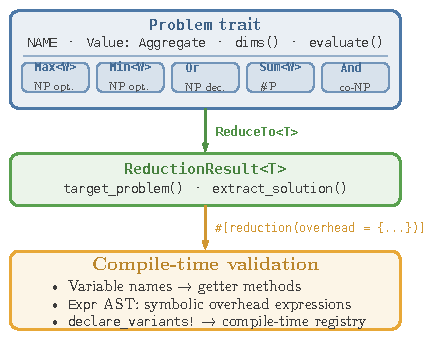
\includegraphics[width=0.5\columnwidth]{figures/architecture.pdf}
  \caption{Trait hierarchy and compile-time validation.
    The \texttt{Problem} trait defines a universal evaluation interface; \texttt{ReduceTo<T>} requires both forward and inverse maps; procedural macros validate overhead expressions and variant registrations at compile time.}
  \label{fig:architecture}
\end{figure}

\paragraph{Problems and variants.}
Every problem type implements \texttt{Problem}, which requires: a constant name, an associated \texttt{Value} type, a method returning the configuration space dimensions, an \texttt{evaluate()} method that maps any configuration to a value, and variant metadata.
The \texttt{Value} type is an \emph{aggregation wrapper} that determines how individual evaluations combine across the configuration space.
Six wrappers cover the standard problem classes (\Cref{tab:wrappers}).
Each wrapper implements an \texttt{Aggregate} trait with \texttt{identity()}, \texttt{combine()}, and optional witness-tracking methods, so a brute-force solver reduces to a single fold over the configuration space: \texttt{configs.map(evaluate).fold(identity, combine)}.
Wrappers that support \emph{witness recovery} can track which configuration achieved the optimal value; those that cannot (counting and co-NP) only produce aggregate values.
This distinction propagates to the reduction traits.

\begin{table}[h]
\caption{Aggregation wrappers and their complexity classes.}\label{tab:wrappers}
\centering
\small
\begin{tabular}{@{}llll@{}}
\toprule
Wrapper & Class & Witness & Example \\
\midrule
\texttt{Max<W>} & NP optimization & Yes & Max.\ Indep.\ Set \\
\texttt{Min<W>} & NP optimization & Yes & Min.\ Vertex Cover \\
\texttt{Or}     & NP decision     & Yes & $k$-Satisfiability \\
\texttt{Sum<W>} & \#P counting    & No  & $k$-th Largest $m$-Tuple \\
\texttt{And}    & co-NP decision  & No  & (reserved) \\
\shortstack[l]{\texttt{Extremum}\\\texttt{<V>}} & NP optimization$^\dagger$ & Yes & Integer Lin.\ Prog. \\
\bottomrule
\end{tabular}
\\[2pt]
{\footnotesize $^\dagger$\texttt{Extremum} differs from \texttt{Max}/\texttt{Min} only in that the optimization sense is chosen at runtime.}
\end{table}
A single problem type admits multiple \emph{variants}: parameterizations by graph type (\texttt{SimpleGraph}, \texttt{PlanarGraph}, \texttt{BipartiteGraph}, \texttt{KingsSubgraph}, \texttt{UnitDiskGraph}, etc.) and weight type (unit, \texttt{i32}, \texttt{f64}).
Each variant may have a better complexity bound---MIS on king's subgraphs runs in $2^{O(\sqrt{|V|})}$~\cite{deBerg2020ETHTight} versus $O(1.1996^{|V|})$ on general graphs~\cite{Xiao2017MIS}.
The \texttt{declare\_variants!} macro registers each concrete instantiation with its best-known complexity, a factory for JSON deserialization, and a solve function.
All variable names in complexity expressions are validated at compile time against the problem's getter methods.
This registry produces the registered variants from 100+ base problem types.

\paragraph{Decision problems.}
A generic \texttt{Decision<P>} wrapper converts any optimization problem \texttt{P} (whose value type is \texttt{Max<W>} or \texttt{Min<W>}) into a decision problem with value type \texttt{Or}: given a bound~$k$, it asks whether a configuration meeting or exceeding~$k$ exists.
The wrapper implements \texttt{Problem} automatically via the \texttt{DecisionProblemMeta} trait, which supplies the decision variant's name.
The reduction from the decision wrapper to its inner optimization type is derived generically, so adding a decision variant requires only a one-line macro invocation (\texttt{register\_decision\_variant!}). 
Three problem types currently have decision variants: Maximum Independent Set, Minimum Vertex Cover, and Minimum Dominating Set.

\paragraph{Reduction rules.}
The type system enforces a split based on witness capability.
\texttt{ReduceTo<T>} requires a \texttt{ReductionResult} that bundles \texttt{target\_problem()} and \texttt{extract\_solution()}, a map from a target \emph{configuration} back to a source configuration.
An agent cannot compile a forward reduction without providing the inverse map; incomplete reductions are compile errors.
\texttt{ReduceToAggregate<T>} requires an \texttt{AggregateReductionResult} with \texttt{extract\_value()} instead, a map from a target \emph{value} back to a source value, with no witness recovered.
Each reduction also carries a compile-time-validated overhead: the \texttt{\#[reduction(overhead = \{...\})]} procedural macro attaches symbolic size expressions, and variable names are checked against getter methods on the source type, so a typo causes a compile error, not a silent bug.

\paragraph{Solvers.}
When the user invokes \texttt{pred solve}, the system selects a solver in priority order.
First, if the problem has a dedicated solver that exploits its structure (currently six problem types), the system uses it.
Second, if a witness-capable reduction path to Integer Linear Programming (ILP) exists, the system reduces along the cheapest path (by Dijkstra) and solves with HiGHS.
Third, the brute-force enumerator is always available: it folds over all configurations using the aggregation interface.
\textcolor{red}{Brute force remains essential for round-trip testing, where correctness matters more than speed.}

\paragraph{Reduction graph construction.}
Problem variants and reduction rules compose into the directed graph described in \Cref{sec:graph-structure}.
For subtype edges (e.g., MIS on a king's subgraph to MIS on a general graph), a generic \texttt{ReductionAutoCast} implements both reduction traits with an identity solution map.
At runtime, type-erased blanket implementations (\texttt{DynReductionResult}) let the reduction-graph engine chain reductions along Dijkstra-discovered paths without knowing the concrete types at compile time.

\section{Solver Coverage: QUBO}\label{app:qubo-coverage}

Specialized hardware for combinatorial optimization is one of the fastest-growing frontiers of AI infrastructure.
Ising machines, quantum annealers~\cite{glover2019}, and physics-inspired neural solvers~\cite{Schuetz2022PhysicsGNN} all promise substantial speedups over conventional CPU solvers, and the field has converged on a single input format: QUBO.
The catch is that the speedup is only available \emph{after} the user has hand-translated their problem into QUBO, a step that has historically required a domain expert per problem and a fresh paper per reduction.
This is exactly where the reduction graph pays off.

Treating QUBO as one registered solver target, \texttt{pred to QUBO -{}-hops 3} reports 138~problem variants that route to it with witness recovery in the current library.
\Cref{tab:qubo-coverage} samples ten and lists the composed overhead $r_{\text{QUBO} \leftarrow A}$, the polynomial mapping source size to QUBO variable count.
All ten share one invocation, \texttt{pred reduce - -{}-to QUBO}, and only the input changes.
By contrast, solver-specific compilers such as PyQUBO~\cite{Zaman2021PyQUBO} and qubovert~\cite{Iosue2022qubovert} accept QUBO input but provide no inter-problem reductions, leaving the translation step to the user.

\begin{table}[htbp]
\caption{Ten problems reaching QUBO within three hops, sampled from 138~reachable variants. A QUBO-capable solver inherits all of them via one command.}
\label{tab:qubo-coverage}
\centering
\small
\begin{tabular}{@{}llll@{}}
\toprule
Problem & Hops & $r_{\text{QUBO} \leftarrow A}$ & Application \\
\midrule
GraphPartitioning           & 1 & $O(V)$              & VLSI partitioning \\
3-Satisfiability            & 1 & $O(C + V)$          & Verification, planning \\
Knapsack                    & 1 & $O(n + b)$          & Resource allocation \\
TravelingSalesman           & 1 & $O(V^2)$            & Logistics, PCB drilling \\
KColoring                   & 1 & $O(V^2)$            & Register allocation \\
Partition                   & 2 & $O(n + b)$          & Load balancing \\
MaximumClique               & 2 & $O(V^3)$            & Bioinformatics \\
BinPacking                  & 2 & $O(n^3)$            & VM/container packing \\
MultiprocessorScheduling    & 2 & $O(P T^2 + P^2 T)$  & Cloud scheduling \\
MaximumIndependentSet       & 3 & $O(V^3)$            & Wireless scheduling \\
\bottomrule
\end{tabular}
\\[2pt]
{\footnotesize $V$: vertices; $C$: clauses; $n$: items; $b$: encoding/slack bits; $P, T$: processors, tasks.}
\end{table}

\newpage
\section{Skill Excerpts}\label{app:skills}

\Cref{fig:skills} reproduces the two skills referenced in \Cref{sec:pipeline-overview}: \texttt{propose} (advisor skill that gates issue creation by domain experts) and \texttt{add-rule} (automation skill that drives implementation from a validated issue).

\begin{figure*}[htbp]
  \centering
  \begin{minipage}[t]{0.525\textwidth}
  \begin{tcolorbox}[
    colback=gray!5, colframe=gray!80,
    title={\textbf{\texttt{propose}} --- advisor skill (excerpts)},
    fonttitle=\footnotesize, boxrule=0.4pt, arc=2pt, left=4pt, right=4pt, top=2pt, bottom=2pt,
    equal height group=skillbox,
  ]
  \footnotesize
  \begin{lstlisting}[basicstyle=\ttfamily\scriptsize, numbers=none, frame=none, aboveskip=0pt, belowskip=0pt, xleftmargin=4pt]
---
name: propose
description:
  Guides domain experts through brainstorm-
  ing and files a GitHub issue
---
  \end{lstlisting}
  \vspace{-4pt}
  \rule{\linewidth}{0.3pt}\\[3pt]
  \textbf{No programming knowledge required.}
  This skill works entirely in mathematical / domain language.\\[3pt]
  %
  \texttt{<HARD-GATE>}\\
  Do NOT write any code, create any files, or invoke implementation skills.
  The ONLY output of this skill is GitHub issues filed via \texttt{gh issue create}.\\
  \texttt{</HARD-GATE>}\\[3pt]
  %
  \rule{\linewidth}{0.3pt}\\[3pt]
  \textbf{Run topology analysis first} to identify the most impactful missing reductions [\ldots]\\
  \begin{lstlisting}[basicstyle=\ttfamily\scriptsize, numbers=none, frame=none, aboveskip=-5pt, belowskip=2pt, xleftmargin=4pt]
cargo run --example \
    detect_isolated_problems
cargo run --example \
    detect_unreachable_from_3sat
  \end{lstlisting}
  \vspace{-2pt}
  \rule{\linewidth}{0.3pt}\\[3pt]
  \textbf{Pre-validation} --- Run \texttt{check-issue} on draft before filing:\\[2pt]
  \begin{tabular}{@{}r@{~}l@{}}
    1. & \textbf{Usefulness} --- does a cheaper reduction path already exist? \\
    2. & \textbf{Effort} --- effort to implement? \\
    3. & \textbf{Correctness} --- do cited references support the claims? \\
    4. & \textbf{Writing quality} --- all symbols defined, examples worked? \\
  \end{tabular}\\[2pt]
  Only issues passing all four checks are filed.
  \end{tcolorbox}
  \label{fig:skill-propose}
  \end{minipage}\hspace{4pt}%
  \begin{minipage}[t]{0.445\textwidth}
  \begin{tcolorbox}[
    colback=gray!5, colframe=gray!80,
    title={\textbf{\texttt{add-rule}} --- automation skill (excerpts)},
    fonttitle=\footnotesize, boxrule=0.4pt, arc=2pt, left=4pt, right=4pt, top=2pt, bottom=2pt,
    equal height group=skillbox,
  ]
  \footnotesize
  \begin{lstlisting}[basicstyle=\ttfamily\scriptsize, numbers=none, frame=none, aboveskip=0pt, belowskip=0pt, xleftmargin=4pt]
---
name: add-rule
description: Adding a new reduction 
  rule to the codebase, either from 
  an issue or interactively
---
  \end{lstlisting}
  \vspace{-4pt}
  \rule{\linewidth}{0.3pt}\\[3pt]
  \textbf{Required Information Checklist}
  \begingroup
  \setlength{\leftmargini}{1.4em}
  \setlength{\itemsep}{1pt}
  \setlength{\parskip}{0pt}
  \begin{enumerate}
    \item \textbf{Reduction algorithm} --- how to transform source instance to target, with BibTeX reference.
    \item \textbf{Size overhead} --- how target size relates to source size, used for estimating the overhead of the reduction.
    \item \textbf{Concrete example} --- a small worked-out instance, used for testing and documentation.
    \item $\ldots$
  \end{enumerate}
  \endgroup
  Do NOT proceed until the checklist is complete.\\[3pt]
  %
  \rule{\linewidth}{0.3pt}\\[3pt]
  \textbf{Reference Implementations} --- Read these first:\\
  {\ttfamily src/rules/mvc\_mis.rs} [\ldots{}]\\[3pt]
  % {\ttfamily src/unit\_tests/rules/\ldots{} (same stem)}\\[3pt]
  %
  \rule{\linewidth}{0.3pt}\\[3pt]
  \textbf{Document in paper.}
  Write a \texttt{reduction-rule} entry in the Typst paper with theorem body, proof (construction, correctness, solution extraction), and a worked example with concrete numbers.
  Run \texttt{make paper} --- must compile without errors.
  \end{tcolorbox}
  \label{fig:skill-addrule}
  \end{minipage}
  \caption{Two skills that bookend the contribution pipeline.
    \textbf{\texttt{propose}} (left) gates issue creation by domain experts: the hard gate enforces no-code contribution, topology analysis guides experts toward strategic reduction-graph gaps, and pre-validation checks four quality dimensions before the issue enters the pipeline.
    \textbf{\texttt{add-rule}} (right) drives implementation from a validated issue: the checklist encodes the mathematical knowledge every reduction requires, reference implementations prevent convention drift, and the paper entry ensures visual verifiability by human reviewers.}
  \label{fig:skills}
\end{figure*}

\newpage
\section{Agent Profile Example}\label{app:agent-profile}

\Cref{fig:agent-profile} shows a representative agent profile used by the \emph{agentic feature tests} described in \Cref{sec:verification}. The persona's domain knowledge lets the sub-agent judge whether reduction outputs are plausible without access to ground-truth labels.

\begin{figure}[h]
  \centering
  \begin{tcolorbox}[
    colback=gray!5, colframe=gray!80,
    title={\textbf{Agent Profile:} Dr.\ Sarah Chen --- CLI Tool (\texttt{pred})},
    fonttitle=\small, boxrule=0.4pt, arc=2pt, left=4pt, right=4pt, top=2pt, bottom=2pt
  ]
  \small
  \textbf{Use case.}
  An algorithm engineer reads the project documentation to learn what problems and reductions exist, then uses the \texttt{pred} CLI to model and solve their own optimization problems.
  Each session: pick a problem from the paper, create an instance with real-world-style data, find a reduction path to a solver, solve it, and verify the result.\\[4pt]
  %
  \textbf{Persona.}
  Senior algorithm engineer at a logistics company with ten years of experience in vehicle routing, scheduling, and layout optimization.
  Knows these problems map to graph coloring, independent set, set cover, and similar NP-hard formulations because she has hand-coded reductions before.
  Found this project's paper and wants to try the CLI instead of writing reductions herself.
  Has never used \texttt{pred} before.\\[4pt]
  %
  \textbf{Behavior.}
  Reads the paper and docs first, then picks a problem she recognizes.
  Figures out the CLI by reading its help output.
  After each step, compares the output against her expectation.
  If something does not match, investigates before moving on.
  \end{tcolorbox}
  \caption{A representative agent profile used in agentic feature testing.
    The persona's domain knowledge (logistics optimization) lets the agent judge whether reduction results are plausible without access to ground-truth labels.}
  \label{fig:agent-profile}
\end{figure}

\section{Development Phases}\label{app:phases}

In Phase~1 (weeks~0--7), the team and AI agents ported reduction rules from existing packages (ProblemReductions.jl~\cite{gao2025programming}, UnitDiskMapping.jl~\cite{Nguyen2023UnitDiskMapping,pan2025encodingcomputationallyhardproblems}, and qubogen~\cite{Tamura2020qubogen}) and from Garey and Johnson's catalogue~\cite{garey1979}.
Growth was steady but slow: roughly 20~problem types and 55~rules by week~7.
Through this process, the skill-based automation pipeline was established and iteratively refined.
In Phase~2 (weeks~7--8.5), basic skills were introduced, but the pipeline was not yet end-to-end automated.
In Phase~3 (weeks~8.5--13), the full pipeline became operational.
Both curves accelerate sharply: problem types grew from 23 to 187, and reduction rules from 52 to 239, in under five weeks.
External domain experts began contributing through the \texttt{propose} skill, filed structured issues in mathematical language while agents handled implementation.

\section{End-User Utility Experiment Details}\label{app:end-user}

This appendix expands on the controlled experiment summarised in \Cref{sec:end-user-utility}.

\paragraph{Setup.}
A Claude Opus~4.7 agent (\texttt{claude-opus-4-7}, dispatched via Claude Code's general-purpose subagent and recorded in each run's \texttt{meta.json}) receives an engineer-voice prompt: a manager splits a 150-person organization into two product teams to maximize total cross-team value from a dense signed pairwise survey (${\approx}\,5300$ entries, density ${\approx}\,0.48$, mix of positive and negative scores).
The prompt gives no model or solver hint; recognizing the underlying signed-weight Max-Cut structure is part of the task.
Configurations form a $2{\times}2$ factorial over \emph{web search} (yes/no) and \emph{\texttt{pred} access} (yes/no), with ten random instances per cell (40 runs) and a 90~s solver wall-time cap.
Agents with \texttt{pred} access also receive a short Markdown protocol that scripts a graph-data-driven reformulation step before solver code is written: \texttt{pred from} enumerates reachable downstream models, \texttt{pred path} reads each candidate's reduction overhead, \texttt{pred show} reads each endpoint's declared worst-case complexity, and \texttt{pred reduce} / \texttt{pred extract} handle the forward and inverse mappings between the natural-model instance and the chosen target endpoint. The protocol prescribes a single-pass external solver call inside an OS-enforced \texttt{timeout 90} and instructs the agent to report whatever the call returns honestly, without any retry-on-poor-result loop. The same single-pass / honest-reporting discipline is also imposed on the bare-AI conditions to keep the four configurations comparable.

\paragraph{Three independent axes of measurement.}
We separate three quantities that AI-coding evaluations often blend into a single ``time'' figure:
(i) \emph{AI cost}---tokens consumed by the agent;
(ii) \emph{algorithm cost}---solver wall-time, reported by the agent in a structured \texttt{meta.json};
(iii) \emph{solution quality}---feasibility and the raw objective value, both re-checked by an independent grader on the original instance literals.

\paragraph{Scope.}
The experiment isolates one mechanism---catalog-driven downstream reformulation---and tests it in a regime where alternative formulations are decisive.
We do not claim the same gains transfer to families where the natural formulation is already strong (sparse ILP, scheduling) or to other agent backends.
The benchmark harness---scenario generator, grader, per-run result schema, and aggregation script---is released alongside the library to support broader replication.

\paragraph{Per-instance solver picks.}
\Cref{tab:end-user-solver-table} lists the solver each agent selected on every instance.
Without \texttt{pred}, the bare baselines drift across MILP (HiGHS, PuLP+CBC), MIQP (Gurobi with \texttt{NonConvex=2}), OR-tools CP-SAT, simulated annealing (\texttt{dwave-neal} / \texttt{dwave-samplers}), \texttt{dwave-tabu}, and ad-hoc local-search heuristics; the misses concentrate on the integer-programming routes whose linear relaxations are weak on dense signed-weight cut maximization.
With \texttt{pred}+web every run routes simulated annealing on the Ising / QUBO endpoint; the offline \texttt{pred} variant likewise routes to simulated annealing on 9 of 10 instances, with the single miss occurring when the agent's training-time priors led it to commit to a 45{,}000-variable MILP route on the \texttt{ILP/bool} endpoint instead.

\begin{table}[h]
\caption{Solver picked on each instance by each configuration.
SA~=~simulated annealing on the Ising / QUBO reformulation (\texttt{dwave-neal} or \texttt{dwave-samplers}); MILP~=~mixed-integer linear program (HiGHS or PuLP+CBC); MIQP~=~mixed-integer quadratic program (Gurobi); CP-SAT~=~OR-tools constraint programming; Tabu~=~D-Wave \texttt{TabuSampler}; Custom~=~hand-rolled local search (KL / ILS / 1-flip multi-start).
Bold cells are the largest gaps to the per-instance best.}
\label{tab:end-user-solver-table}
\centering
\small
\begin{tabular}{@{}c@{\hspace{2pt}}llll@{}}
\toprule
Seed & Bare AI         & Bare AI + web   & + \texttt{pred}   & + \texttt{pred} + web \\
\midrule
 7 & \textbf{CP-SAT}   & SA              & SA & SA \\
11 & SA                & \textbf{MILP}   & SA & SA \\
13 & \textbf{MILP}     & MIQP            & MIQP & SA \\
17 & \textbf{MILP}     & SA              & SA & SA \\
19 & Custom            & \textbf{MILP}   & SA & SA \\
23 & SA                & MIQP            & SA & SA \\
29 & SA                & SA              & SA & SA \\
31 & SA                & MIQP            & Custom SA & SA \\
37 & SA                & MIQP            & \textbf{MILP} & SA \\
41 & Tabu              & SA              & SA & SA \\
\midrule
\textbf{solver families} & 4 & 4 & 3 & 1 \\
\bottomrule
\end{tabular}
\end{table}

\paragraph{Raw per-run data.}
\Cref{tab:end-user-raw-obj} lists the objective achieved by each (configuration, instance) pair, and \Cref{tab:end-user-raw-wall} the corresponding solver wall-times. Bold cells in \Cref{tab:end-user-raw-obj} mark misses below the per-instance best.

\begin{table}[h]
\caption{Raw per-instance objective for each configuration. The right column is the per-instance best across the four configurations; bold cells fall below it.}
\label{tab:end-user-raw-obj}
\centering
\small
\begin{tabular}{@{}cccccc@{}}
\toprule
Seed & Bare AI & Bare AI + web & + \texttt{pred} & + \texttt{pred} + web & Best \\
\midrule
 7 & \textbf{12{,}656} & 12{,}962          & 12{,}962         & 12{,}962 & 12{,}962 \\
11 & 12{,}641          & \textbf{10{,}011} & 12{,}641         & 12{,}641 & 12{,}641 \\
13 & \textbf{11{,}673} & 12{,}944          & 12{,}944         & 12{,}944 & 12{,}944 \\
17 & \textbf{12{,}182} & 12{,}326          & 12{,}326         & 12{,}326 & 12{,}326 \\
19 & 12{,}915          & \textbf{10{,}252} & 12{,}915         & 12{,}915 & 12{,}915 \\
23 & 12{,}240          & 12{,}240          & 12{,}240         & 12{,}240 & 12{,}240 \\
29 & 12{,}944          & 12{,}944          & 12{,}944         & 12{,}944 & 12{,}944 \\
31 & 12{,}401          & 12{,}401          & 12{,}401         & 12{,}401 & 12{,}401 \\
37 & 12{,}471          & 12{,}471          & \textbf{10{,}194}& 12{,}471 & 12{,}471 \\
41 & 12{,}187          & 12{,}187          & 12{,}187         & 12{,}187 & 12{,}187 \\
\midrule
\textbf{mean} & 12{,}431 & 12{,}074 & 12{,}375 & \textbf{12{,}603} & 12{,}603 \\
\bottomrule
\end{tabular}
\end{table}

\begin{table}[h]
\caption{Raw per-instance solver wall-time (seconds) for each configuration. The 90~s OS-enforced kill cutoff is the upper bound; entries near 80--90~s indicate the solver was running until killed.}
\label{tab:end-user-raw-wall}
\centering
\small
\begin{tabular}{@{}ccccc@{}}
\toprule
Seed & Bare AI & Bare AI + web & + \texttt{pred} & + \texttt{pred} + web \\
\midrule
 7 & 75.1 & 26.7 &  1.5 &  5.9 \\
11 & 11.8 & 80.0 &  2.7 &  4.7 \\
13 & 80.2 & 70.0 & 80.0 &  4.7 \\
17 & 75.1 & 11.5 & 17.8 &  4.7 \\
19 & 86.0 & 80.1 &  8.5 &  3.0 \\
23 & 18.5 & 80.2 &  1.2 &  1.6 \\
29 & 24.9 &  2.3 &  2.1 &  5.8 \\
31 & 17.7 & 80.1 & 23.8 & 29.4 \\
37 & 32.0 & 80.1 & 84.7 &  5.9 \\
41 & 60.0 & 30.5 &  3.4 &  1.2 \\
\midrule
\textbf{mean} & 48.1 & 54.2 & 22.6 & \textbf{6.7} \\
\bottomrule
\end{tabular}
\end{table}

%%%%%%%%%%%%%%%%%%%%%%%%%%%%%%%%%%%%%%%%%%%%%%%%%%%%%%%%%%%%

\newpage
\input{checklist.tex}


\end{document}